En la figura \ref{fig:arquitecturaSistema} se muestra el diagrama de componentes que ilustra el como esta compuesta la arquitectura del sistema con cada uno de sus respectivos módulos.

\begin{figure}[h]
    \centering
    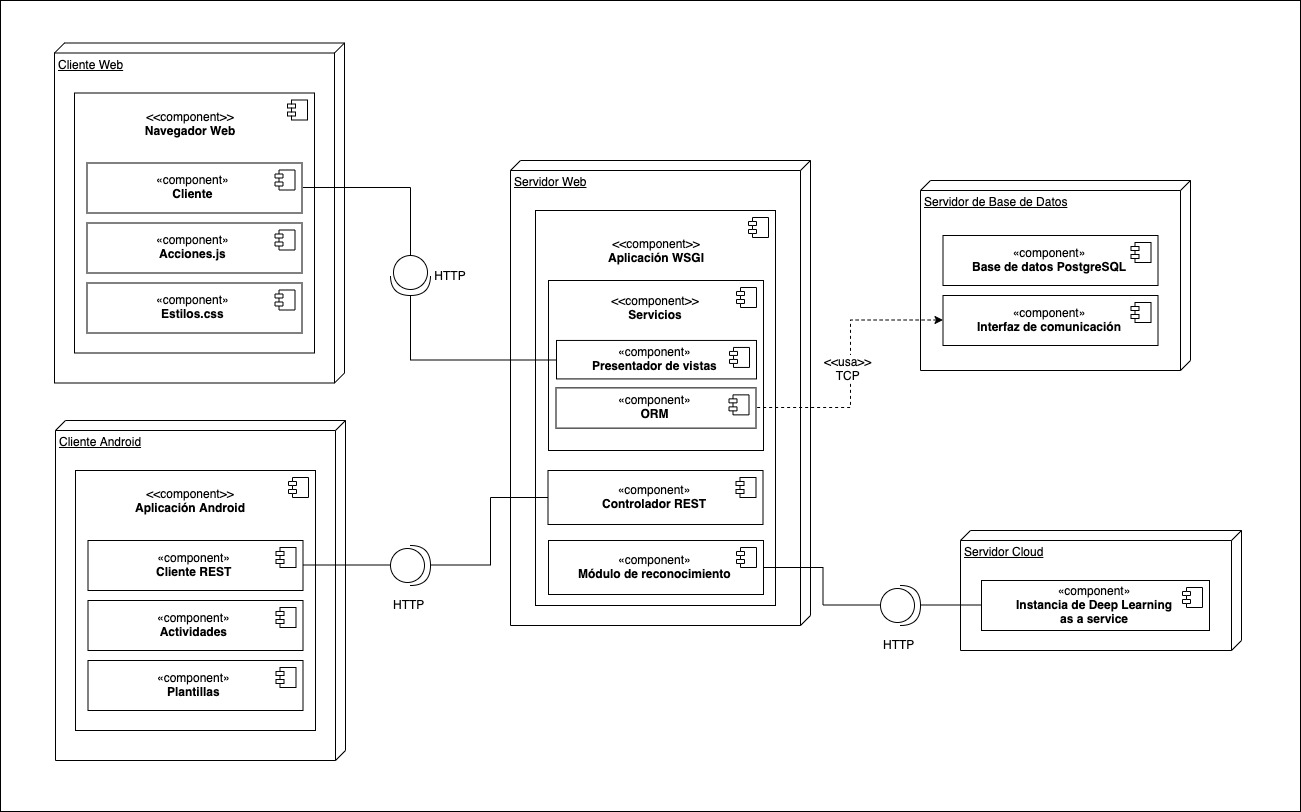
\includegraphics[width=\textwidth]{capitulo4/imagenes/ArquitecturaApp.jpg}
    \caption{Arquitectura del sistema.}
    \label{fig:arquitecturaSistema}
\end{figure}
\subsection{Cliente web}
En el cliente web se tienen las páginas web desarrolladas con el motor de templates de Django, además, para mejorar la interacción que tiene el usuario con el sistema se incluyen recursos como lo son scripts de Javascript para el control de acciones y los archivos de estilos CSS.
\subsection{Cliente android}
En la parte de Android se tiene un cliente REST para llevar a cabo las peticiones y controlar las respuestas del servidor web, se tiene las actividades y plantillas XML para la interfaz de usuario junto con los casos de uso que controlan la lógica del sistema.
\subsection{Servidor web}
En el servidor web es donde se tendrán los componentes para conectar el resto de módulos entre si, es decir, por un lado tenemos el presentador de vistas de Django para controlar al cliente web, para la interacción con el servidor web se utiliza directamente el ORM de Django para evitar lidiar con querys y seguir con un desarrollo orientado a objetos,  se tienen los serializadores para la interacción con el cliente REST de a Android que también hace uso de los modelos de Django y que en conjunto controlan las peticiones y resultados del API REST, por último se tiene el módulo de reconocimiento que de forma más precisa funciona como un cliente que consume y realiza peticiones al servidor web con el modelo para el reconocimiento y traducción de expresiones matemáticas.
\subsection{Servidor de base de datos}
El sistema gestor de base de datos se encontrará en su propio servidor para separarlo de del servidor web, se desarrollará en postgreSQL y con ello permitir que el sistema este mejor modularizado y tener una independencia en capa complemente de la arquitectura.
\subsection{Servidor cloud}
Servidor cloud es en dónde se realizará la tarea de realizar la traducción a \LaTeX{}  mediante el uso de redes neuronales cómo se estableció con anterioridad, el utilizar este tipo de servicio que proporciona Amazon, Google o Microsoft permite evitar lidiar con problemas de infraestructura y despliegue. Además hace que el entrenamiento sea más sencillo debido a los recursos que  nos proporcionan.